\documentclass{article}
\usepackage{amsmath,amsfonts}
\usepackage{graphicx}
\usepackage{hyperref}
\usepackage[margin=0.75in]{geometry}

\begin{document}

%------------------------------------------------
% Title: Centered, slightly larger, minimal vspace
%------------------------------------------------
\begin{center}
\Large\textbf{Math 252 -- \S 5.5 Question 4}
\end{center}
\vspace{-2 cm}

%------------------------------------------------
% Table and region image side by side at the top
% Minipages are vertically centered relative to each other.
% Content within each minipage is horizontally centered.
%------------------------------------------------
\begin{figure}[h!]
  \begin{minipage}[c]{0.35\textwidth} % Use [c] for vertical centering of the minipage box
    \centering % Center content (table and caption) within this minipage
    \[
    \begin{array}{|c|c||c|c|}
    \hline
    \textstyle f(x_0) & \textstyle f(0) &         & 0   \\ \hline
    \textstyle f(x_1) & \textstyle f(1) & A       & 3.1 \\ \hline
    \textstyle f(x_2) & \textstyle f(2) & B       & 4.5 \\ \hline
    \textstyle f(x_3) & \textstyle f(3) & C       & 4.3 \\ \hline
    \textstyle f(x_4) & \textstyle f(4) & D       & 6.7 \\ \hline
    \textstyle f(x_5) & \textstyle f(5) & E       & 6.0 \\ \hline
    \textstyle f(x_6) & \textstyle f(6) &         & 0   \\ \hline
    \end{array}
    \]
    \caption*{\small Distances across the region\\at 1 cm intervals}
  \end{minipage}\hfill
  \begin{minipage}[c]{0.6\textwidth} % Use [c] for vertical centering of the minipage box
    \centering % Center content (image and caption) within this minipage
    
\includegraphics[width=\linewidth]{region4.png}
    \vspace{-2.6cm} % Adjust this value or remove if caption spacing is okay
    \caption*{\small Vertical distances measured\\across the intervals}
  \end{minipage}
\end{figure}

\vspace{10pt} % Separation from the figure above

%------------------------------------------------
% Simpson's Rule calculation with interpretation
%------------------------------------------------
\large\textbf{Interpreting the Table and Applying Simpson's Rule:}

The table provides measurements across the region. To apply Simpson's Rule, we must identify our interval and parameters:
\begin{align}
a &= 0,\quad b = 6,\quad n = 6 \text{ (even, as required)} \notag\\
\Delta x &= \frac{b-a}{n}=\frac{6-0}{6}=1 \text{ cm} \notag\\
x_k &= a+k\Delta x = 0, 1, 2, 3, 4, 5, 6 \quad \text{for } k=0,1,\ldots,6 \notag
\end{align}

The table gives us the values A, B, C, D, E which represent $f(1)=3.1$, $f(2)=4.5$, $f(3)=4.3$, $f(4)=6.7$, $f(5)=6.0$. The endpoints are $f(0)=0$ and $f(6)=0$ (region touches the x-axis at both ends).

\vspace{5pt}
\[
\int_{0}^{6} f(x)\,dx
\;\approx\;
\frac{\Delta x}{3}
\Bigl[
    f(0)+4f(1)+2f(2)+4f(3)+2f(4)+4f(5)+f(6)
\Bigr]
\]
\vspace{5pt}
\begin{align}
&= \frac{1}{3}\bigl[0+4(3.1)+2(4.5)+4(4.3)+2(6.7)+4(6.0)+0\bigr] \notag\\
&= \frac{1}{3}(12.4 + 9.0 + 17.2 + 13.4 + 24.0) = \frac{76.0}{3} = \mathbf{25.33} \text{ cm}^2 \notag
\end{align}

%------------------------------------------------
% Parabolic illustration at bottom
%------------------------------------------------
\begin{figure}[h!]
  \centering
  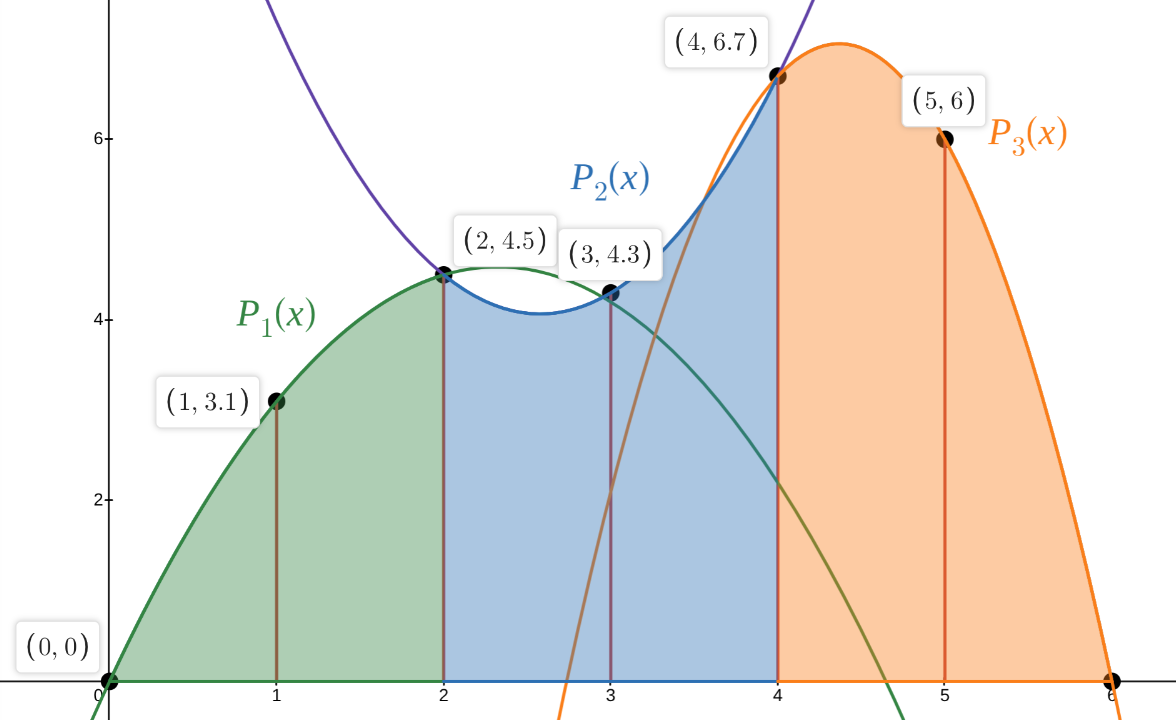
\includegraphics[width=0.4\linewidth]{sec5-5-q4.png} % Reduced width
  \caption*{\small Three parabolas (each spanning two sub‑intervals) illustrating Simpson's Rule approximation. \quad
           Interactive version available at
           \href{https://www.desmos.com/calculator/zeb7iuxly2}{desmos.com/calculator/zeb7iuxly2}.}
\end{figure}

\end{document}
